\section*{Uvod}

Mašinsko učenje je postalo sastavni deo softvera koji svakodnevno koristimo i na koji se oslanjamo. U ovoj disertaciji definišemo novu porodicu algoritama dubokog mašinskog učenja gde podrazumevamo rad sa dubokim neuronskim mrežama, danas najnaprednijim algoritmima mašinskog učenja. Nova porodica modela koju nazivamo negativni modeli ili modeli negativnog dubokog učenja namenjeni su kao nadogradnje postojećih modela. Svrha ovih novodefinisanih modela je da poboljšaju performanse postojećih modela uvođenjem dodatnog negativnog znanja u proces treniranja. Negativni modeli predstavljeni u ovoj disertaciji mogu biti korišćeni kao čiste nadogradnje postojećih modela a biće prikazano kakav je njihov uticaj na performanse u situacijama koje mogu biti problematične čak i za najnaprednije modele današnjice kao što su okluzije, delimični ulazni podaci, šum u ulaznim podacima i slično.

\section*{Negativno duboko učenje}

Pre same definicije negativnih modela potrebno je da definišemo šta se podrazumeva pod negativnim učenjem. Negativno učenje je pojam koji se često koristi u psihologiji pogotovo kod izučavanja ponašanja gde se negativno učenje često izjednačava sa kažnjavanjem u procesu učenja. \cite{mcleod2007bf,staddon2003operant} Naša definicija se razlikuje od ove definicije po tome što mi u sferi mašinskog učenja i dubokog učenja definišemo negativno učenje na jednostavniji način: kao ponašanje do kojeg ne želimo da dođe. Ovakva definicija najlakše se objašnjava na primeru. Kod problema klasifikacije pod negativnim učenjem podrazumevamo način na koji možemo modelu i algoritmu za treniranje tog modela defisati koji podaci ne odgovaraju određenim klasama. Kod problema regresije, na sličan način definišemo negativne podatke (negativne paterne) kao one kojima treniramo model na takav način da izlazni podaci ne treba da "liče" na neki negativan patern. 

U agentskim okruženjima definicija je ista kao definicija psihologije kažnjavanja ili negativnih nagrada koju smo spomenuli iznad. Drugim rečima, kod modeliranja algoritama namenjenih radu u agentskim okruženjima, modeliramo dedukciju gde je naša pretpostavka da će agent koji u svim situacijama zna šta ne treba da uradi, na kraju izvršiti akciju koja vodi ka optimalnom rešenju.

U nekim algoritmima, definisaćemo i pojam negativnih osobina, kao osobine ili specifičnosti ulaznih podataka na osnovu kojih znamo kako izlazni podaci ne treba da izgledaju.

Osim prednosti koje smo spomenuli kao što je potencijalno uvećanje performansi, negativni modeli imaju i drugih prednosti. Na primer, moguće je postojanje problema za koje postoje samo negativni podaci (na primer, kod agenata). U takvim scenarijima bitno je koristiti algoritme koji znaju da obrade negativne podatke kako bi njihova primena bila uspešna. Drugi razlog, kojim ćemo se najviše baviti u okviru ove disertacije je povećana robustnost negativnih modela. Stepen robustnosti definišemo kao osobinu algoritama mašinskog učenja koja nam govori koliko je trenirani model otporan na razne izmene (namerne ili nenamerne) ulaznih podataka. U okviru ove disertacije pokazaćemo kako se negativni modeli ponašaju u nekim teškim situacijama i kako takve situacije utiču na performanse modela dubokog učenja. Jedan primer je adversarijalno učenje \cite{goodfellow2014generative} gde se modeli mogu izučavati i gde možemo generisati podatke sa specifičnom namenom koja vodi ka greškama u predviđanju izlaznih podataka. Kao što ćemo pokazati u ovoj disertaciji, negativni modeli u većini situacija imaju veću otpornost na razne adversarijalne napade i druge oblike izmenjenih ulaznih podataka.

\section*{Modeli negativnog dubokog učenja}

Modele negativnog dubokog učenja definišemo kao modele koji mogu da na neki nač koriste negativne podatke. Negativni podaci mogu biti definisani na više načina kao što su nedostajući podaci, obrnuti podaci, pogrešni podaci, podaci sa šumom, adversarijalni podaci i slično. Specifičnost negativnih dubokih modela ogleda se u tome što mogu da ove negativne podatke koriste kako dodatne informacije u svom obučavanju. Procesi obučavanja zahtevaju specifične izmene kako bi negativni podaci mogli biti upotrebljeni.

\subsection*{Mogući modeli}

Prvi negativni model koji spominjemo je model koji koristi nedostajuće ili negativne osobine. \cite{milovsevic2019classification} Negativne osobine definišemo kao osobine (paterne) ulaznih podataka za koje znamo da postoje ali koji nisu prisutni u određenim ulaznim podacima. Sve neuronske mreže koriste pozitivne osobine kako bi "zapamtile" određene paterne u ulaznim podacima koji se kasnije koriste za buduća predviđanja. Čak i u ovim modelima, nedostatak neke osobine (koji se ogleda u niskoj aktivaciji specifičnih neurona) se takođe uzima u obzir prilikom zaključivanja. Negativne osobine kod negativnih modela se proglašavaju najvažnijim osobinama, i to je najvažnija razlika ovih modela kada ih poredimo sa tracionalnim modelima dubokih neuronskih mreža. Može se reći da negativni modeli uče i trenirani su na takav način da koriste dedukciju gde će moći da zaključuju na osnovu osobina koje znamo da postoje ali trenutno nisu prisutne. Ovo je pogotovo važno kod specifičnih problema kao što su klasifikacija delimičnih ulaza, na primer kod klasifikacije slika. Ljudima je veoma prirodno da u ovakvim problemima koriste dedukciju gde će znanjem o ostalim slikama i postojećim klasama moći da nadomeste nedostajuće podatke na slici koju trenutno posmatraju. Modeli koji koriste nedostajuće osobine pokušavaju da modeliraju ovakav način razmišljanja.

Drugi model koji je sličan i koji spominjemo je model treniran na osnovu parcijalnih (negativnih) ulaznih podataka. Primoravanjem modela na ovakav način treniranja očekujemo da će se paterni u ulaznim podacima naučiti na takav način gde će znanje biti upotrebljivo čak i kod kompletnih ulaznih podataka. Negativnost ovih modela dolazi iz činjenice da je lako definisati i da parcijalni ulazi ne pripadaju nekim klasama (kod problema klasifikacije). Na taj način, veštačkim putem dobijamo negativne podatke koji nam i ovde služe za profinjenje modela koje bi vodilo povećanim performansama. 

Negativni podaci, pored načina koji smo upravo opisali, mogu da se dobiju i na još jedan sličan način. Definišemo model koji uči negativne izlazne podatke. Ovakav pristup je najčistiji i najnaivniji pristup negativnom dubokom učenju. Kod ovakvog učenja kod problema klasifikacije, u toku treniranja neuronskoj mreži dajemo ulazne podatke i klase kojima ti podaci ne pripadaju. Odabir klase (ili klasa) kojima podaci ne pripadaju može biti dobro definisan ili nasumičan (češće korišćen). Implementacija ovakvog pristupa nije jednostavna jer zahteva određene izmene kod samog algoritma učenja gde se funkcija greške (eng. loss function) definiše na takav način da ne želimo da je minimizujemo u procesu gradijentnog spusta kao što je slučaj u normalnom treniranju. Ovde koristimo gradijentni uspon gde pokušavamo da se što više udaljimo od negativne izlazne klase.

Još jedan model o kom ćemo kasnije biti više detalja je takozvani spojeni (eng. Ensemble Learning) model. Spojeni modeli su modeli koji se sastoje iz više samostalnih modela. Iako negativni modeli rade dobro, što se može videti iz naših eksperimenata, u nekim situacijama je bolje ukoliko ih koristimo u kombinaciji sa normalnim (pozitivnim) modelima. \cite{milosevic2020synergy} Ova osobina otkrivena je dubljom analizom modela za klasifikaciju na osnovu nedostajućih osobina, gde je uočeno da negativni modeli pored generalno bolje preciznosti u procesu negativnog učenja izgube deo znanja koji pozitivni modeli poseduju. Kombinacijom pozitivnog i negativnog modela dobijamo još veću preciznost.

\subsection*{Klasifikacija na osnovu nedostajućih osobina}

Prvi model koji analiziramo je model za klasifikaciju na osnovu nedostajućih osobina (CBOMF model). \cite{milovsevic2019classification} Sve konvolutivne neuronske mreže u problemima klasifikacije koriste pozitivne ili prisutne osobine kako bi odlučile koja je ispravna izlazna klasa. Novina CBOMF modela je što radi upravo obrnuto -- koristi nedostajuće osobine u ulaznim podacima kako bi zaključio koja je ispravna izlazna klasa. Ova ideja je nastala intuitivno iz ljudskog ponašanja. Na primer, kada ljudi klasifikuju slike, često je poželjno gledati i koje osobine (boje, teksture, objekti) nedostaju na slikama i ako su sve izlazne klase poznate, često je moguće dedukcijom zaključiti o čemu se radi. Jedan primer ovakvog razmišljanja možemo videti na slici \ref{fig:sample-motivation}. 

\begin{figure}[htp]
\centering
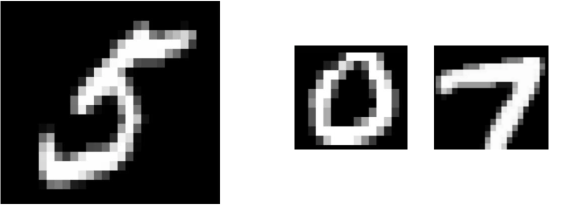
\includegraphics[height=2cm]{figures/motivation.pdf}

{Ponovljena Slika~\ref{fig:sample-motivation}: Motivacioni primer gde je klasifikacija na osnovu negativnih osobina moguća. Slika cifre 5 iz MNIST skupa podataka i njene dve nedostajuće osobine. Osobina 1 (levo) prisutna je u ciframa 0, 6, 8 i 9 dok je osobina 2 (desno) prisutna u ciframa 1, 2, 3, 4, i 7. Nedostatak ove dve osobine u negativnom modelu znači da posmatramo primerak cifre 5.} 
\end{figure}

Naše modifikacije postojećih modela imitiraju ovaj proces. Rezultati koje ćemo prikazati pokazuju da je ovakav trening prvenstveno moguć sa implementacione strane, i da vodi ka modelima koji imaju povećanu robustnost. Proces koji je opisan u ovoj disertaciji može biti primenjen na bilo koju konvolutivnu neuronsku mrežu bez dodatnih podataka.

Upotreba ovakvih modela može imati vrlo široku primenu, pogotovo u problemima klasifikacije slika, na koje se i mi fokusiramo u ovoj disertaciji. Povećana robustnost je veoma važna u kritičnim sistemima kao što su na primer autonomni automobili. Kod autonomne vožnje agent (najčešće duboka neuronska mreža u kombinaciji sa drugim algoritmima) upravlja vozilom na osnovu niza senzora i kamera na vozilu. Kamere koje se koriste daju sliku visoke rezolucije kako bi sistem mogao uočiti objekte na putu. U svakodnevnoj upotrebi, sa druge strane, lako se može desiti da su važni objekti (npr. saobraćajni znaci) na neki način sakriveni, iza drugih objekata kao što su drveće, drugi automobili i slično. Sistem mora imati sposobnost da neometano radi i u ovakvom okruženju, odnosno da je sposoban da, na primer, prepozna o kom se saobraćajnom znaku radi na osnovu delimične slike istog, slično kako i vozači rade u svakodnevnom životu.

Implementacija ovakvog modela počinje sa definicijom jednog negativnog skupa podataka čija je namena testiranje negativnih modela u teškim situacijama. U našim prvim eksperimentima koristili smo MNIST \cite{lecun1998mnist} skup rukom pisanih cifara, koji smo proširili sa dodatnim validacionim skupovima. MNIST skup podataka sadrži 60000 slika za trening i 10000 slika za validaciju, dok se naš prošireni skup nazvan PMNIST (eng. Partial MNIST, delimični MNIST) sastoji od ovih 70000 slika i dodatnih 40000 validacionih slika. Četiri dodatna validaciona skupa dodata su kako bismo bili u mogućnosti da testiramo kako se negativni modeli ponašaju u problemima klasifikacije parcijalnih ulaza. Primeri slika iz validacionih skupova mogu se videti na slici \ref{fig:dsexamples}.

\begin{figure}[htp]
  \centering
  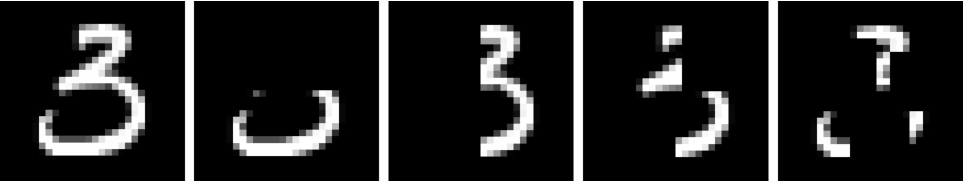
\includegraphics[height=2cm]{datasetimages}
  
  {Ponovljena slika \ref{fig:dsexamples}: Primer validacionih skupova PMNIST skupa podataka. Primer cifre 3 iz validacionog skupa sa modifikacijama, sa leva na desno: originalna slika, horizontalno sečena slika, vertikalno sečena slika, dijagonalno sečena slika i "triple cut" slika u kojoj su uklonjena tri kvadrata dimenzija 9x9 piksela.}
\end{figure}

Isti proces ponvoljen je i na EMNIST \cite{cohen2017emnist} skupu podataka koji pored cifara sadrži i rukom pisana slova engleske abecede. Za testiranje je odabran model sa relativno jednostavnom arhitekturom iz repozitorijuma biblioteke za rad neuronskim mrežama PyTorch. \cite{paszke2017pytorch} Neuronska mreža ima dva konvolutivna sloja i jedan skriveni povezani sloj. U kasnijim testiranjima korišćen je i napredniji Residual Network (ResNet) model kako bismo ispitali kako se naše izmene ponašaju kod upotrebe sa najnaprednijim modelima današnjice. 

Da bismo mogli koristiti zaključivanje na osnovu negativnih osobina moramo implementirati izmene u samoj arhitekturi modela kroz uvođenje negativne aktivacione funkcije. Ova modifikacija se implementira negacijom postojeće aktivacione funkcije čiji rezultat je niz postojećih osobina u ulaznom paternu. Ovaj niz možemo zamisliti kao niz fiksne dužine gde su postojeće osobine predstavljene vrednostima blizu $ 1 $ a nedostajuće osobine imaju vrednost blizu $ 0 $. Pozicija negacije je izuzetno bitna. Aktivaciona funkcija se negira samo jednom i to na prelazu iz konvolutivnih slojeva u povezane (guste, eng. Dense, Fully-Connected) slojeve. U tom trenutku signal koji prolazi kroz neuronsku mrežu predstavlja upravo niz ekstrahovanih osobina koji smo spomenuli i njegovom negacijom dobijamo negativne osobine. Proces negacije zavisi od aktivacione funkcije korišćene u poslednjem konvolutivnom sloju. Posmatramo koje su moguće izlazne vrednosti (i njihovo značenje) i definišemo funkciju negacije koja će na neki način obrnuti izlazne vrednosti. Na primer ukoliko se koristi sigmoidna ili ReLU funkcija, funkcija negacije \( f(x) = 1 - x \) u našim eksperimentima daje dobre rezultate.

Za implemntaciju ove izmene korišćena je dinamična priroda PyTorch biblioteke za rad sa neuronskim mrežama gde je dovoljno modifikovati samo "forward" funkciju koja definiše kako se signal propagira unapred. Operacije za učenje i propagaciju unazad nije bilo neophodno menjati.

Važno je napomenuti da osobine o kojima govorimo nisu binarne ($0$  ili $1$) već su to realne vrednosti. Vrednosti negativnih osobina gotovo nikad nisu tačno $0$ već su to niske vrednosti kojima mi dajemo veću važnost. Važno je napomenuti i da proces koji smo opisali negira sve osobine, i da postoji mogućnost da se detekcijom i negacijom samo osobina relevantnim za određene klase može doći do još boljih rezultata. To je pravac istraživanja koji tek treba biti istražen.

Proces treniranja negativnih modela je sličan klasičnom treniranju neuronskih mreža sa manjim izmenama. Dve najvažnije izmene su treniranje u više faza i zamrzavanje konvolutivnih slojeva. Treniranje u više faza podrazumeva da se za treniranje negativnih modela koriste postojeći konvolutivni slojevi iz pozitivnih modela. Ovaj korak je neophodan kod poređenja pozitivnih i negativnih modela kako bismo bili sigurni da je naša izmena u arhitekturi dovela do promene performansi a ne neki drugi faktor. Drugim rečima želimo da poredimo modele koji detektuju iste osobine: pozitivni modeli rade sa postojećim osobinama a negativni modeli rade sa nedostajućim osobinama.

U eksperimentalnoj fazi testirani su i negativni modeli koji ne koriste višefazno treniranje (ONN model) ali ovi modeli ne predstavljaju ono što je bila namera: da se iste osobine ekstrahuju a zatim negiraju. Ukoliko ne koristimo višefazno treniranje, treniranjem mreža dobićemo kompletno druge osobine (konvolutivne filtere).

Svi ostali negativni modeli (HN, ALT, NR) koje ćemo prikazati koriste višefazno treniranje i zamrzavanje konvolutivnih slojeva. Zamrzavanje konvolutivnih slojeva je još jedan način da se osiguramo da se prilikom treniranja negativnih modela konstantno koriste iste osobine. U suprotnom došlo bi do izmena parametara ovih slojeva i negativni i pozitivni modeli bi bili neuporedivi. Važno je spomenuti da prilikom poređenja negativnih i pozitivnih modela uvek koristimo modele iste arhitekture (osim negacije propagiranog signala kod negativnih modela) sa istim brojem skrivenih neurona i drugim parametrima. Takođe, koristimo iste hiperparametre kao što su broj epoha, korak učenja i slično. Radi lakšeg razumevanja sledi kratak opis četiri modela za koje prikazujemo rezultate

\begin{itemize}
    \item ONN - only negative network: negativni model koji ne koristi zamrzavanje konvolutivnih slojeva i višefazno treniranje. Ovaj model koristi samo negaciju aktivacione funkcije na izlasku iz poslednjeg konvolutivnog sloja.
    \item HN - hybrid network: negativni model koji koristi negativnu aktivacionu funkciju, višefazno treniranje i zamrzavanje konvolutivnih slojeva.
    \item NR - no reset: model isti kao HN model koji ne koristi resetovanje povezanih slojeva u višefaznom treniranju
    \item ALT - alternating: model koji koristi naizmenično treniranje između pozitivne i negativne aktivacione funkcije.
\end{itemize}

Prvo prikazujemo rezultate treniranja na neizmenjenom MNIST skupu podataka. Cilj ovog testa bio je da ispitamo da li je uopšte moguće trenirati negativne modele na način koji smo opisali. Rezultati se mogu videti u tabeli \ref{tab:results-unmodified} gde je vidljivo da negativni modeli koje smo opisali mogu biti trenirani da koriste negativne osobine uz veoma slične (visoke) performanse u poređenju sa pozitivnim modelima iste arhitekture.

\begin{table}[ht]
  \centering
  \begin{tabular}{rS[table-format=2.1]S[table-format=2.1]S[table-format=2.1]S[table-format=2.1]S[table-format=2.1]S[table-format=2.1]}
    \toprule
     \textit{Dataset/Model} & SN & ONN & HN & NR & ALT \\
    \midrule
    {MNIST} & {99.13} & {98.90} & {99.18} & {99.21} & {99.05} \\
    {EMNIST-MNIST} & {99.18} & {99.07} & {99.16} & {99.15} & {99.00} \\
    {EMNIST-Balanced} & {87.14} & {87.62} & {87.38} & {86.78} & {87.92} \\
    
    \bottomrule
  \end{tabular}
  {\vskip 0cm Ponovljena tabela \ref{tab:results-unmodified}: Rezultati testiranja na nepromenjenim skupovima podataka.}
\end{table} 

Sledeći rezultati u tabeli \ref{tab:results-final} prikazuju kako se modeli ponašaju u situacijama kada postoje parcijalni ulazi. Celi rezultati svih modela mogu se pronaći u disertaciji, dok ovde prikazujemo samo najbolje modele gde je jasno vidljivo da se u skoro svim slučajevima negativni modeli bolje snalaze sa parcijalnim ulazima.

\begin{table}[ht]
  \centering
  \begin{tabular}{rS[table-format=12.1]S[table-format=32.1]S[table-format=42.1]}
    \toprule
     \textit{Dataset} & {Best model} & {Accuracy} & {Delta} \\
    \midrule
    {Unmodified - PMNIST}  & {NR} & {99.21} & {0.08} \\
    {Horizontal cut - PMNIST} & {NR} & {56.07} & {11.36} \\
    {Vertical cut - PMNIST} & {ALT} & {69.66} & {12.20} \\
    {Diagonal cut - PMNIST} & {ALT} & {62.49} & {9.52} \\
    {Triple cut - PMNIST} & {ALT} & {46.40} & {5.72} \\
    {Unmodified - EMNIST-MNIST} & {HN} & {99.16} & {-0.02} \\
    {Horizontal cut - EMNIST-MNIST} & {HN} & {54.76} & {5.69} \\
    {Vertical cut - EMNIST-MNIST} & {HN} & {32.91} & {1.81} \\
    {Diagonal cut - EMNIST-MNIST} & {ALT} & {61.50} & {3.07} \\
    {Triple cut - EMNIST-MNIST} & {HN} & {53.90} & {7.12} \\
    {Unmodified - EMNIST-Balanced} & {ALT} & {87.92} & {0.78} \\
    {Horizontal cut - EMNIST-Balanced} & {ONN} & {26.97} & {6.02} \\
    {Vertical cut - EMNIST-Balanced} & {ALT} & {24.36} & {2.13} \\
    {Diagonal cut - EMNIST-Balanced} & {HN} & {30.79} & {2.88} \\
    {Triple cut - EMNIST-Balanced} & {ONN} & {22.88} & {2.49} \\
    
    \bottomrule
  \end{tabular}
  {Ponovljena tabela \ref{tab:results-final}: Prikaz najboljih modela za sve validacione skupove. "Accuracy" kolona prikazuje preciznost na kraju treninga dok "Delta" kolona prikazuje razliku između prikazanog negativnog modela i pozitivnog modela iste arhitekture. Obe kolone predstavljaju procente korektno klasifikovanih validacionih slika.}
\end{table}

Prilikom testiranja modela i procesa, testirane su razne modifikacije opisanog procesa:

\begin{itemize}
    \item Testiranje uticaja višefaznog treniranja: Kako bismo bili sigurni da je naša modifikacija negacije osobina dovela do povećanih performansi a ne sam proces višefaznog treniranja, napravljen je ekspirement gde je višefazno treniranje upotrebljeno nad običnim pozitivnim modelima. Nisu uočene greške u našem procesu a višefazno treniranje je u nekim slučajevima čak imalo negativan uticaj na preciznost modela.
    \item Testiranje negativnih konvolutivnih filtera: Umesto negacije aktivacione funkcije, takođe je eksperimentisano i sa negacijom samih konvolutivnih filtera. Eksperimentalno je pokazano da ovakva izmena ne dovodi do izmene rezultata negativnih modela te da je moguće koristiti umesto negacije aktivacione funkcije.
    \item Druge aktivacione funkcije: Pored testiranja modela koji koriste danas najčešće korišćene ReLU aktivacione funkcije, eksperimentima je utvrđeno da je moguće negirati i $ sigmoid $, $ tanh $, $LeakyReLU$ i $ReLU6$ aktivacione funkcije bez većih izmena u rezultatima.
    \item Okluzije: Pored validacije sa parcijalnim ulazima, negativni modeli su testirani i sa okluzijama i to sa ugaonim okluzijama od 10 do 50 odsto. I kod ovakvog tipa nedostajućih podataka, negativni modeli daleko nadmašuju performanse običnih modela.
\end{itemize}

Posebno interesantni eksperimenti su eksperimenti sa adversarijalnim napadima. Negativni modeli opisani u ovoj disertaciji testirani su i sa white-box i sa black-box adversarijalnim napadima. Razlika ove dve vrste napada ogleda se u tome koliko je napadaču informacija dostupno prilikom generisanja adversarijalnih podataka. Kod black-box napada napadač je ograničen i nema znanje o arhitekturi mreže dok se kod white-box napada napadaču omogućava pristup svim parametrima (pogotovo gradijentima) napadnutih modela. Korišćeni su FGSM (Fast Gradient Sign Method) \cite{goodfellowexplaining} white-box napad i PGD (Projected Gradient Descent) \cite{madry2017towards} napad na negativne modele gde su pokazali povećanu otpornost na ove tipove napada u odnosu na klasične modele. Primer poređenja može se videti na slici \ref{fig:fgsm_chart} gde poredimo klasičan i negativni model, oba napadnuta FGSM napadom.

\begin{figure}
    \centering
    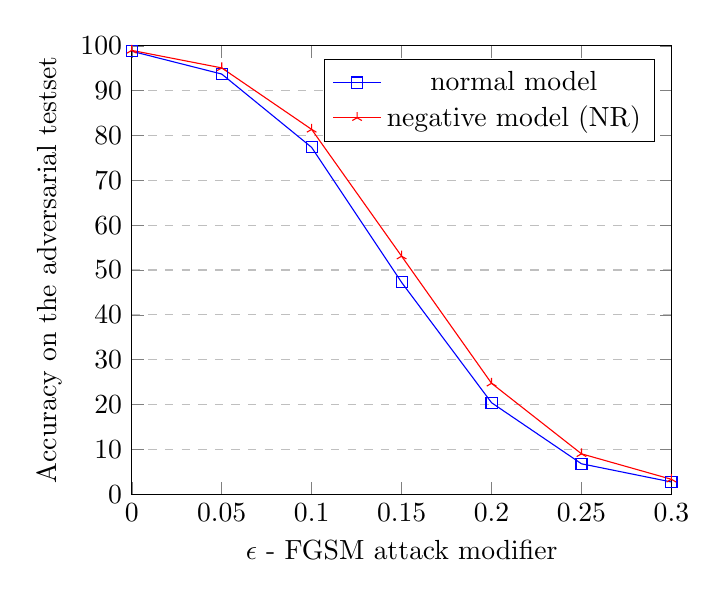
\begin{tikzpicture}
    \begin{axis}[
        xlabel={\(\epsilon\) - FGSM attack modifier},
        ylabel={Accuracy on the adversarial testset},
        xmin=0, xmax=0.3,
        ymin=0, ymax=100,
        xtick={0,0.05,0.1,0.15,0.2,0.25,0.3},
        ytick={0,10,20,30,40,50,60,70,80,90,100},
        legend pos=north east,
        ymajorgrids=true,
        grid style=dashed,
        xticklabels={0,0.05,0.1,0.15,0.2,0.25,0.3}
    ]
    
    \addplot[
        color=blue,
        mark=square,
        ]
        coordinates {
        (0,98.79)(0.05,93.70)(0.1,77.34)(0.15,47.23)(0.2,20.39)(0.25,6.77)(0.3,2.71)
        };
        \addlegendentry{normal model}
        
    \addplot[
        color=red,
        mark=Mercedes star, % lewis hamilton bre
        ]
        coordinates {
        (0,98.98)(0.05,95.07)(0.1,81.35)(0.15,53.07)(0.2,24.72)(0.25,8.99)(0.3,3.31)
        };
        \addlegendentry{negative model (NR)}
        
    \end{axis}
    \end{tikzpicture}
    {\newline Ponovljena slika \ref{fig:fgsm_chart}: Preciznost normalnog i negativnog (NR) modela napadnutih FGSM adversarijalnim napadom za razne faktore napada ($ \epsilon$)}
    
\end{figure}

\subsection*{Sinergija negativnog i klasičnog učenja}

Negativni modeli opisani u ovoj disertaciji doprinose na preciznosti i robustnosti u teškim i adversarijalnim situacijama, kao što smo pokazali. Međutim, ovi modeli imaju još jednu karakteristiku a to je da dodatne performanse koje proizilaze iz dodatnog negativnog znanja nisu pravi nadskup znanja koje poseduju normalni modeli. Drugim rečima, povećan broj ispravno klasifikovanih primera nam govori da su negativni modeli generalno bolji od običnih modela neuronskih mreža, ali daljim ispitivanjem slučajeva može se utvrditi da postoje slučajevi u kojima normalna mreža radi bolje od negativne mreže. Da bi se ovaj nedostatak nadomestio, predlažemo arhitekturu sinergije, spajanje dva modela istih arhitektura gde je jedan pozitivan a drugi negativan. Deo težina, odnosno parametri konvolutivnih slojeva su deljeni dok se parametri povezanih skrivenih slojeva čuvaju odvojeno za pozitivan i negativan deo. Arhitektura modela može se videti na slici \ref{fig:1}. 

\begin{figure}
  \centering
  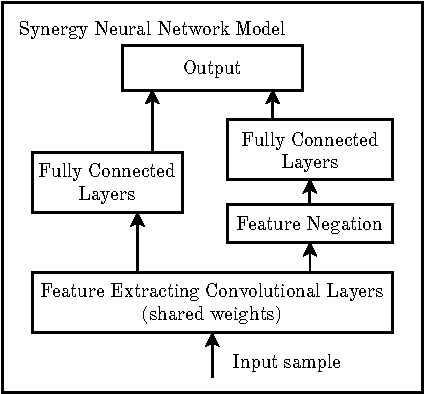
\includegraphics{figures/fig1.pdf}
  {\centering \vskip 0cm Ponovljena slika \ref{fig:1}: Arhitektura sinergije.}
\end{figure}

Ispitavanjem broja korektno klasifikovanih slučajeva može se videti da postoji mogućnost za implementaciju modela viših performansi ukoliko bi se napravio spoj modela. Naime, ispitan je broj slučajeva u kojima je makar jedna od dve ispitivane mreže imala tačnu izlaznu klasu i uočeno je da je taj broj veći od broja ispravno klasifikovanih validacionih slučajeva oba pojedinačna modela. Na CIFAR-10 skupu podataka, teoretska preciznost spojene mreže bi bila $ 74.54\% $.

Implementacija sinergije je jednostavna jer su oba modela već unapred trenirana na način koji smo opisali u prethodnom poglavlju. Model sinergije ne zahteva nikakvo dodatno treniranje. Važna napomena je da se izlazni podaci oba modela moraju spojiti i da postoji više načina na koji se modeli mogu spojiti. Najjednostavniji način koji je korišćen je izračuvanje zbira verovatnoća po klasama koje nam daju oba modela. Razlog upotrebe ovakvog spoja je intuicija da je u slučajevima gde dolazi do pogrešne klasifikacije razlika verovatnoća za ispravnu klasu i pogrešnu klasu koja je krajnji rezultat veoma mala i da se dodavanjem verovatnoća drugog modela ova greška može ispraviti. Ovakvi slučajevi postoje i najbolje je pokazati na primeru o čemu se radi. Jedan primer može se videti u tabeli \ref{tab:3} gde je normalna mreža pogrešno klasifikovala jedan primer, dok je negativna mreža bila ispravna. Zbir rezultata u modelu sinergije ponovo vodi ka tačnoj klasifikaciji. Postoje slučajevi i kada je obrnuto: normalna mreža ispravno klasifikuje a negativna mreža pogrešno klasifikuje. Postoje i ekstremni slučajevi gde su obe mreže pogrešno klasifikovale primer a sinergija odnosno zbir te dve mreže ispravno klasifikovala primer, što se može videti u tabeli \ref{tab:5}.

\begin{table}
\centering
{Ponovljena tabela \ref{tab:3}: Jedan slučaj kada je samo jedna mreža ispravno klasifikovala primer iz validacionog skupa (na poziciji \#2). C1 do C10 su verovatnoće po klasama. Ispravna klasa je klasa 9 -- 'brod'. Redovi predstavljaju tri mreže: normalnu, negativnu, i sinergiju kao zbir prethodne dve. Podebljanim tekstom obeležene su najviše verovatnoće.}

\tabcolsep=0.04cm
\begin{tabular}{lrrrrrrrrrr}
\hline\noalign{\smallskip}
 & C1 & C2 & C3 & C4 & C5 & C6 & C7 & C8 & \textbf{C9} & C10 \\
\noalign{\smallskip}\hline\noalign{\smallskip}
Nor. & 3.05 & \textbf{4.44} & -1.25 & -2.72 & -0.83 & -2.12 & -2.45 & -3.31 & 2.01 & 2.62 \\
Neg. & 6.04 & 7.29 & -1.39 & 0.11 & -6.85 & -8.49 & -9.60 & -4.89 & \textbf{11.55} & 3.22 \\
Syn. & 9.09 & 11.73 & -2.65 & -2.60 & -7.68 & -10.61 & -12.05 & -8.21 & \textbf{13.56} & 5.84 \\
\noalign{\smallskip}\hline
\end{tabular}
\end{table}

\begin{table}
\centering
{Ponovljena tabela \ref{tab:5}: Ekstremni slučaj (\#6418) gde su obe mreže pogrešile, ali sinergija modela daje tačan rezultat. Ispravna klasa je klasa 1 -- 'avion'.}
\tabcolsep=0.06cm
\begin{tabular}{lrrrrrrrrrr}
\hline\noalign{\smallskip}
 & \textbf{C1} & C2 & C3 & C4 & C5 & C6 & C7 & C8 & C9 & C10 \\
\noalign{\smallskip}\hline\noalign{\smallskip}
Nor. & 3.52 & \textbf{4.45} & -0.67 & -2.84 & 1.20 & -2.38 & -2.50 & -3.34 & -0.41 & 0.83 \\
Neg. & 4.00 & 2.63 & -0.31 & -0.16 & \textbf{5.22} & -2.03 & -1.94 & -2.73 & 0.42 & -1.30 \\
Syn. & \textbf{7.53} & 7.07 & -0.97 & -3.00 & 6.43 & -4.41 & -4.44 & -6.07 & 0.01 & -0.48 \\
\noalign{\smallskip}\hline
\end{tabular}
\end{table}

Pored modela sinergije u disertaciji opisujemo i druge slične modele. Svrha nekih od modela su validacija pristupa, na primer imamo model trenirane sinergije koji ima istu arhitekturu kao sinergija ali se trenira na uobičajeni način. Poenta ovakvog modela je da vidimo da li se jednostavnim povećanjem broja parametara može doći do sličnih performansi ili je naš pristup ispravan.

Rezultati modela sinergije mogu se videti u tabeli \ref{tab:6}. Kod modela sinergije korišćen je kompleksniji CIFAR-10 skup slika u boji gde su ponovljeni rezultati opisani u prethodnom delu a koji se odnose na negativne modele. Kod samog negativnog modela vidimo veoma mali porast u preciznosti dok je kod sinergije taj porast dosta veći. Takođe vidimo da se jednostavnim povećanjem broja parametara ne dobija isti rezultat čak i kod upotrebe istih konvolutivnih slojeva (hot-start trenirana sinergija) što vodi ka zaključku da su naša intuicija i proces implementacije ispravni.

\begin{table}
\centering
{Ponovljena tabela \ref{tab:6}: Validaciona preciznost modela u procentima. Kolona "Delta" predstavlja razliku između novih modela (negativnih i sinergije) i normalnog modela. \vskip 0cm}
\begin{tabular}{lcr}
\hline\noalign{\smallskip}
Model & Accuracy & Delta\\
\noalign{\smallskip}\hline\noalign{\smallskip}
Normal & 63.30 & - \\
Negative & 63.57 & 0.27 \\
Synergy & 66.98 & 3.68 \\
Trained Synergy & 63.32 & 0.02 \\
Trained Synergy (hot-start) & 64.28 & 0.98 \\
\noalign{\smallskip}\hline
\end{tabular}
\end{table}

Još jedan validacioni eksperiment je izveden gde je ispitano kako se izmene opisane ovde mogu primeniti na moderne modele neuronskih mreža koji imaju visoku složenost. Testirana je ResNet18 \cite{he2016deep} arhitektura gde se mogu videti slični rezultati kao i za naš jednostavniji model. Iako je dobitak na preciznosti minimalan važno je napomenuti da testirani model već ima izuzetno visoku preciznost od preko $90\%$ pa nije realistično očekivati velika unapređenja. Svakako, pokazano je da našim modifikacijama moguće popraviti čak i najnaprednije modele današnjice. Rezultati se mogu videti u tabeli \ref{tab:7}.

\begin{table}
\centering
{Ponovljena tabela \ref{tab:7}: Validaciona preciznot modela zasnovanih na ResNet18 modelu.}
\vskip 1mm
\begin{tabular}{lcr}
\hline\noalign{\smallskip}
Model & Accuracy & Delta\\
\noalign{\smallskip}\hline\noalign{\smallskip}
Normal & 92.52 & - \\
Negative & 92.48 & -0.04 \\
Synergy & 92.54 & 0.02 \\
Trained Synergy & 89.47 & -3.05 \\
Trained Synergy (hot-start) & 92.46 & -0.06 \\
\noalign{\smallskip}\hline
\end{tabular}
\end{table}

Kao i kod negativnih modela, fokus je bio takođe i na robustnosti. Iz tog razloga model sinergije testiran je i sa parcijalnim i sa adversarijalnim validacionim skupovima. Sažetak eksperimenata je sledeći:

\begin{itemize}
    \item Za testiranje modela sinergije korišćeno je više vrsta okluzija. Ugaone okluzije od $10$ do $30$ procenata, zatim nasumični i fiksirani crni kvadrati varijabilnih dimenzija na slikama. U svim slučajevima model sinergije je nadmašio i normalne modele i negativne modele kao što se može videti u poglavlju \ref{partial}. Na slici \ref{fig:fgsm_chart_synergy} može se videti poređenje normalne mreže i modela sinergije protiv FGSM white-box napada.
    \item Kod adversarijalnih primera korišćen je veći broj white-box i black-box napada: FGSM, PGD, BIM, CW, RFGSM, FFGSM, TPGD, MIFGSM gde je sinergija u svim situacijama imala veći nivo otpornosti na napade u poređenju sa običnim modelima.
\end{itemize}

\begin{figure}
    \centering
    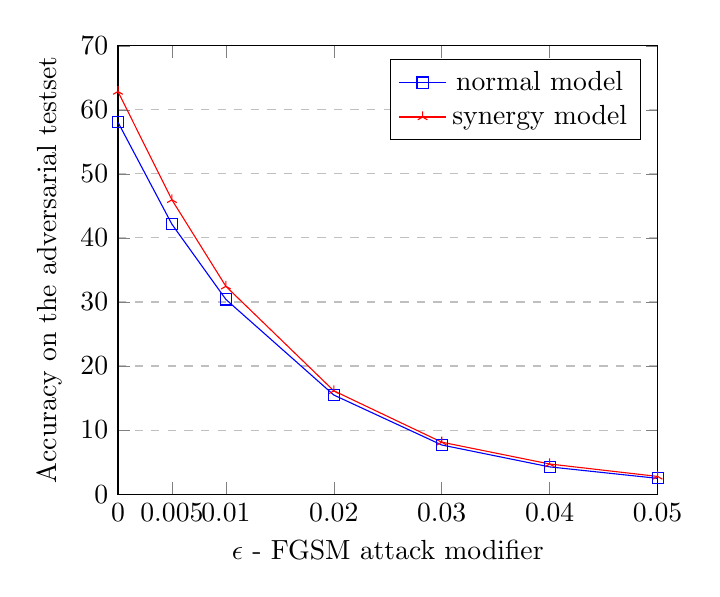
\begin{tikzpicture}
    \begin{axis}[
        xlabel={\(\epsilon\) - FGSM attack modifier},
        ylabel={Accuracy on the adversarial testset},
        xmin=0, xmax=0.05,
        ymin=0, ymax=70,
        xtick={0,0.005,0.01,0.02,0.03,0.04,0.05},
        ytick={0,10,20,30,40,50,60,70},
        legend pos=north east,
        ymajorgrids=true,
        grid style=dashed,
        xticklabels={0,0.005,0.01,0.02,0.03,0.04,0.05},
        log ticks with fixed point,
        scaled x ticks = false
    ]
    
    \addplot[
        color=blue,
        mark=square,
        ]
        coordinates {
        (0,58.07)(0.005,42.14)(0.01,30.40)(0.02,15.47)(0.03,7.67)(0.04,4.25)(0.05,2.46)
        };
        \addlegendentry{normal model}
        
    \addplot[
        color=red,
        mark=Mercedes star, % lewis hamilton bre
        ]
        coordinates {
        (0,62.86)(0.005,45.95)(0.01,32.45)(0.02,16.13)(0.03,8.11)(0.04,4.70)(0.05,2.76)
        };
        \addlegendentry{synergy model}
        
    \end{axis}
    \end{tikzpicture}
    {\vskip 0cm Ponovljena slika \ref{fig:fgsm_chart_synergy}: Preciznost normalnog modela i modela sinergije protiv FGSM napada.}
\end{figure}

Takođe su izvedeni i eksperimenti za različite načine spajanja pozitivne i negativne mreže:

\begin{itemize}
    \item Prosto sabiranje verovatnoća kako je već opisano, prošireno je hiperparametrom $ \omega $ koji definiše u kojem stepenu koji deo mreže utiče na krajnji rezultat. U našim eksperimentima uočene su veoma male razlike za razne vrednosti ovog hiperparametra.
    \item Spajanje množenjem verovatnoća je takođe testirano, bez velikih razlika u odnosu na sabiranje. Ideja između množenja verovatnoća je da će se visoke verovatnoće eksponencijalno uvećati u rezultatu sinergije dok će se manje verovatnoće poništiti.
    \item Dodatni slojevi takođe mogu biti dodati na spoju dve mreže kao nelinearni način spajanja. Moguće je koristiti jedan ili više skrivenih slojeva ili čak konvolutivne slojeve. Prisup sa jednodimenzionalnim konvolutivnim slojem najviše obećava i eliminiše potrebu za odabirom načina spajanja jer se on može naučiti kroz standarni proces učenja i treniranja neuronskih mreža. 
\end{itemize}

\subsection*{Pravo negativno učenje}

Na kraju predstavljamo "prave" negativne modele, odnosno modele koji koriste negativne podatke prilikom treniranja. Problem ovih modela je što zahtevaju specifične slučajeve korišćenja gde su negativni podaci prirodno dostupni ili se mogu lako izgenerisati na veštački način. Iz ovog razloga većina ovakvih modela spomenutih u ovoj disertaciji su predstavljeni kao inicijalne verzije algoritama sa veoma malo testiranja.

Jedan primer koji ćemo istraživati u budućem radu je kod klasifikacije slika. Ukoliko bi postojao skup podataka negativno ručno obeleženih slika odnosno kombinacija slika i klasa kojima ne pripadaju, onda bi se ti podaci mogli koristiti za negativno treniranje. U teoriji ovakav model bi generalizovao isto ili bolje u poređenju sa običnim modelom, pogotovo u situacijama gde imamo parcijalne ulaze.

U ovoj disertaciji predstavljamo dva implementirana modela: Negativnu sijamsku Triplet-Loss mrežu i negativnog DRL (Deep Reinforcement Learning) agenta. Takođe prikazujemo i neke modele koji su još uvek u idejnoj fazi. Ciljevi svih ovih modela su slični kao i za modele koje smo prethodno definisali: da koriste dodatno negativno znanje radi povećanja performansi i robusnosti.

Modeli koji koriste Gradient Ascent (gradijentni uspon) su prvi kandidat za prave negativne modele. Gradient Ascent se koristi u nekim adversarijalnim napadima (npr. FGSM) kako bi model naterao da pogreši modifikacijom gradijenata tako da vode ka pogrešnoj klasi. Gradient Ascent modeli mogu da koriste isti ovaj koncept u kombinaciji sa negativnim podacima da "odvuku" svoje parametre od pogrešne klase koja je data kao negativni primer. Još jedan koncept koji bi mogao biti iskorišćen je negativni sampling podataka. To je proces u kom se skup trening podataka transformiše u negativni skup podataka. Naime, za svaki podatak u skupu zna se ispravna klasa (u problemima klasifikacije) i veštački samim tim se znaju i sve pogrešne (negativne klase). Iteracijom kroz skup i biranjem nasumičnih pogrešnih klasa može se generisati veštački negativni skup podataka.

Prvi implementirani model pravog negativnog učenja koji predstavljamo je negativna sijamska mreža. Sijamske neuronske mreže \cite{koch2015siamese} su specifične po tome što uče sličnost ulaznih paterna. Sijamska arhitektura podrazumeva dve mreže koje su trenirane da predstave podatke u kompresovanom obliku a zatim se posmatra sličnost tih oblika i na osnovu te sličnosti donosimo zaključke. Ovakvi modeli imaju razne prednosti u poređenju sa običnim modelima, na primer, prilikom dobijanja novih podataka nije potrebno trenirati ceo model ispočetka. Zbog ove osobine koriste se već duže vreme za identifikaciju ljudi na osnovu fotografija \cite{varior2016gated}, između ostalog. Sijamske mreže takođe ne zahtevaju velike skupove podataka za treniranje, što je isto velika prednost.

Postoji posebna kategorija sijamskih mreža na koju se fokusiramo, takozvane Triplet sijamske mreže. Ove mreže prilikom treniranja uče sličnosti (radi klasifikacije) između ulaznih podataka (isto kao i ostale sijamske mreže) ali koristi uređene trojke podataka. Koriste tri ulazna podatka: glavni podatak koji se obrađuje, nasumično odabrani podatak iste klase i nasumično odabrani podatak negativne (nasumične pogrešne) klase. Ovakve mreže pokušavaju da učenjem minimizuju razlike u sličnosti između određenog podatka i pozitivnog primerka a maksimizuju razlike između istog određenog podatka i negativnog primerka. 

Naši eksperimenti sa ovim mrežama podrazumevaju scenario gde se negativni primerak koristi kao osnovni izvor znanja. U našim eksperimentima pokušana su dva pristupa. Prvi pristup je da se u potpunosti eliminiše pozitivna strana sijamske arhitekture, ali taj eksperiment dovodi do nemogućnosti mreže da konvergira. Jednostavno rečeno, nasumično treniranje sa negativnim klasama možda nikada neće dovesti do konvergencije modela. Drugi pristup je da se čisto negativno učenje koristi samo kao tehnika za fine-tuning (dodatni trening) modela. U ovom pristupu već trenirani sijamski model se unapređuje korišćenjem čistog negativnog učenja, što je slično našem pristupu kod ostalih modela. Ovaj pristup je ispitan i zaključeno je da je može dovesti do poboljšanja performansi i prevenciji overfitting-a u treniranju. Rezultati se mogu videti na slici \ref{fig:snn_chart}.

\begin{figure}
    \centering
    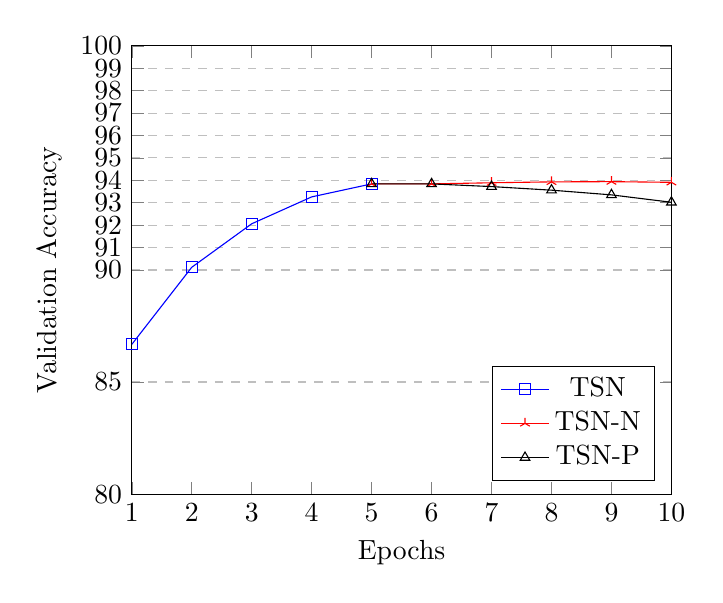
\begin{tikzpicture}
    \label{chart:fgsm}
    \begin{axis}[
        xlabel={Epochs},
        ylabel={Validation Accuracy},
        xmin=1, xmax=10,
        ymin=80, ymax=100,
        xtick={1,2,3,4,5,6,7,8,9,10},
        ytick={80,85,90,91,92,93,94,95,96,97,98,99,100},
        legend pos=south east,
        ymajorgrids=true,
        grid style=dashed,
        xticklabels={1,2,3,4,5,6,7,8,9,10}
    ]
    
    \addplot[
        color=blue,
        mark=square,
        ]
        coordinates {
        (1,86.68)(2,90.12)(3,92.06)(4,93.26)(5,93.84)
        };
        \addlegendentry{TSN}
        
    \addplot[
        color=red,
        mark=Mercedes star, % lewis hamilton bre
        ]
        coordinates {
        (5,93.84)(6,93.84)(7,93.89)(8,93.93)(9,93.94)(10,93.91)
        };
        \addlegendentry{TSN-N}
        
    \addplot[
        color=black,
        mark=triangle,
        ]
        coordinates {
        (5,93.84)(6,93.84)(7,93.72)(8,93.56)(9,93.35)(10,93.02)
        };
        \addlegendentry{TSN-P}
        
    \end{axis}
    \end{tikzpicture}
    {\vskip 1cm Ponovljena slika \ref{fig:snn_chart}: Poređenje finetuning pristupa kod sijamskih triplet-loss neuronskih mreža. TSN je neizmenjena sijamska mreža, TSN-N je ista mreža gde se pozitivna strana zanemaruje prilikom finetuning-a, TSN-P je ista mreža gde se negativna strana zanemaruje prilikom finetuning-a. TSN-N mreža uspeva da poveća svoju preciznost dok TSN-P mreža ne uspeva. Konačne preciznosti su: 93.84\% (TSN), 92.92\% (TSN-P), 93.91\% (TSN-N).}
\end{figure}

Drugi implementirani model je negativni Deep Reinforcement Learning (DRL) agent. U treniranju DRL agenata veoma je važan koncept nagrade gde agent pokušava da optimizuje svoje ponašanje kako bi se nagrada uvećala. U ovom konceptu takođe postoji i druga strana a to je koncept kazne u slučaju da agent pogreši. Naša ideja da ispitamo da li se agenti mogu trenirati koristeći samo negativne nagrade (kazne). U ovom scenariju agent nikada nije nagrađen već uvek bira onu akciju za koju je kazna najmanja. Drugim rečima, agent je treniran da se fokusira na akcije "koje ne treba da uradi". Jedan primer u kojem možemo ispitati ovakvo ponašanje je izbegavanje prepreka gde je agent treniran da izbegava prepreke koje su nasumično generisane i usmerene prema poziciji agenta u dvodimenzionalnom svetu. Ovakav sistem je direktno primenljiv na mnoga druga okruženja na primer na automonomne automobile. Za eksperiment je korišćen DQN \cite{mnih2013playing} agent gde je isti treniran na način da izbegava nasumično generisane prepreke. Ovo okruženje je pogodno za ovakav eksperiment jer često ne postoji specifična akcija koju agent treba da uradi već samo akcije koje agent ne treba da uradi. Agent ima četiri moguće akcije odnosno četiri smera u kojima može da se kreće: gore, dole, levo i desno. Kako agent nikad nije nagrađen, kumulativna vrednost nagrade $ 0 $ je najbolji mogući rezultat. 

Zaključak eksperimenta je da je ovakav način treniranja negativnih agenata moguć i primenljiv na razne probleme koje ćemo istražiti u budućem istraživanju. Test okruženje je moguće videti na slici \ref{fig:bird}, dok se rezultati (nagrade) mogu videti na slici \ref{fig:birdr}.

\begin{figure}[!ht]
  \centering
  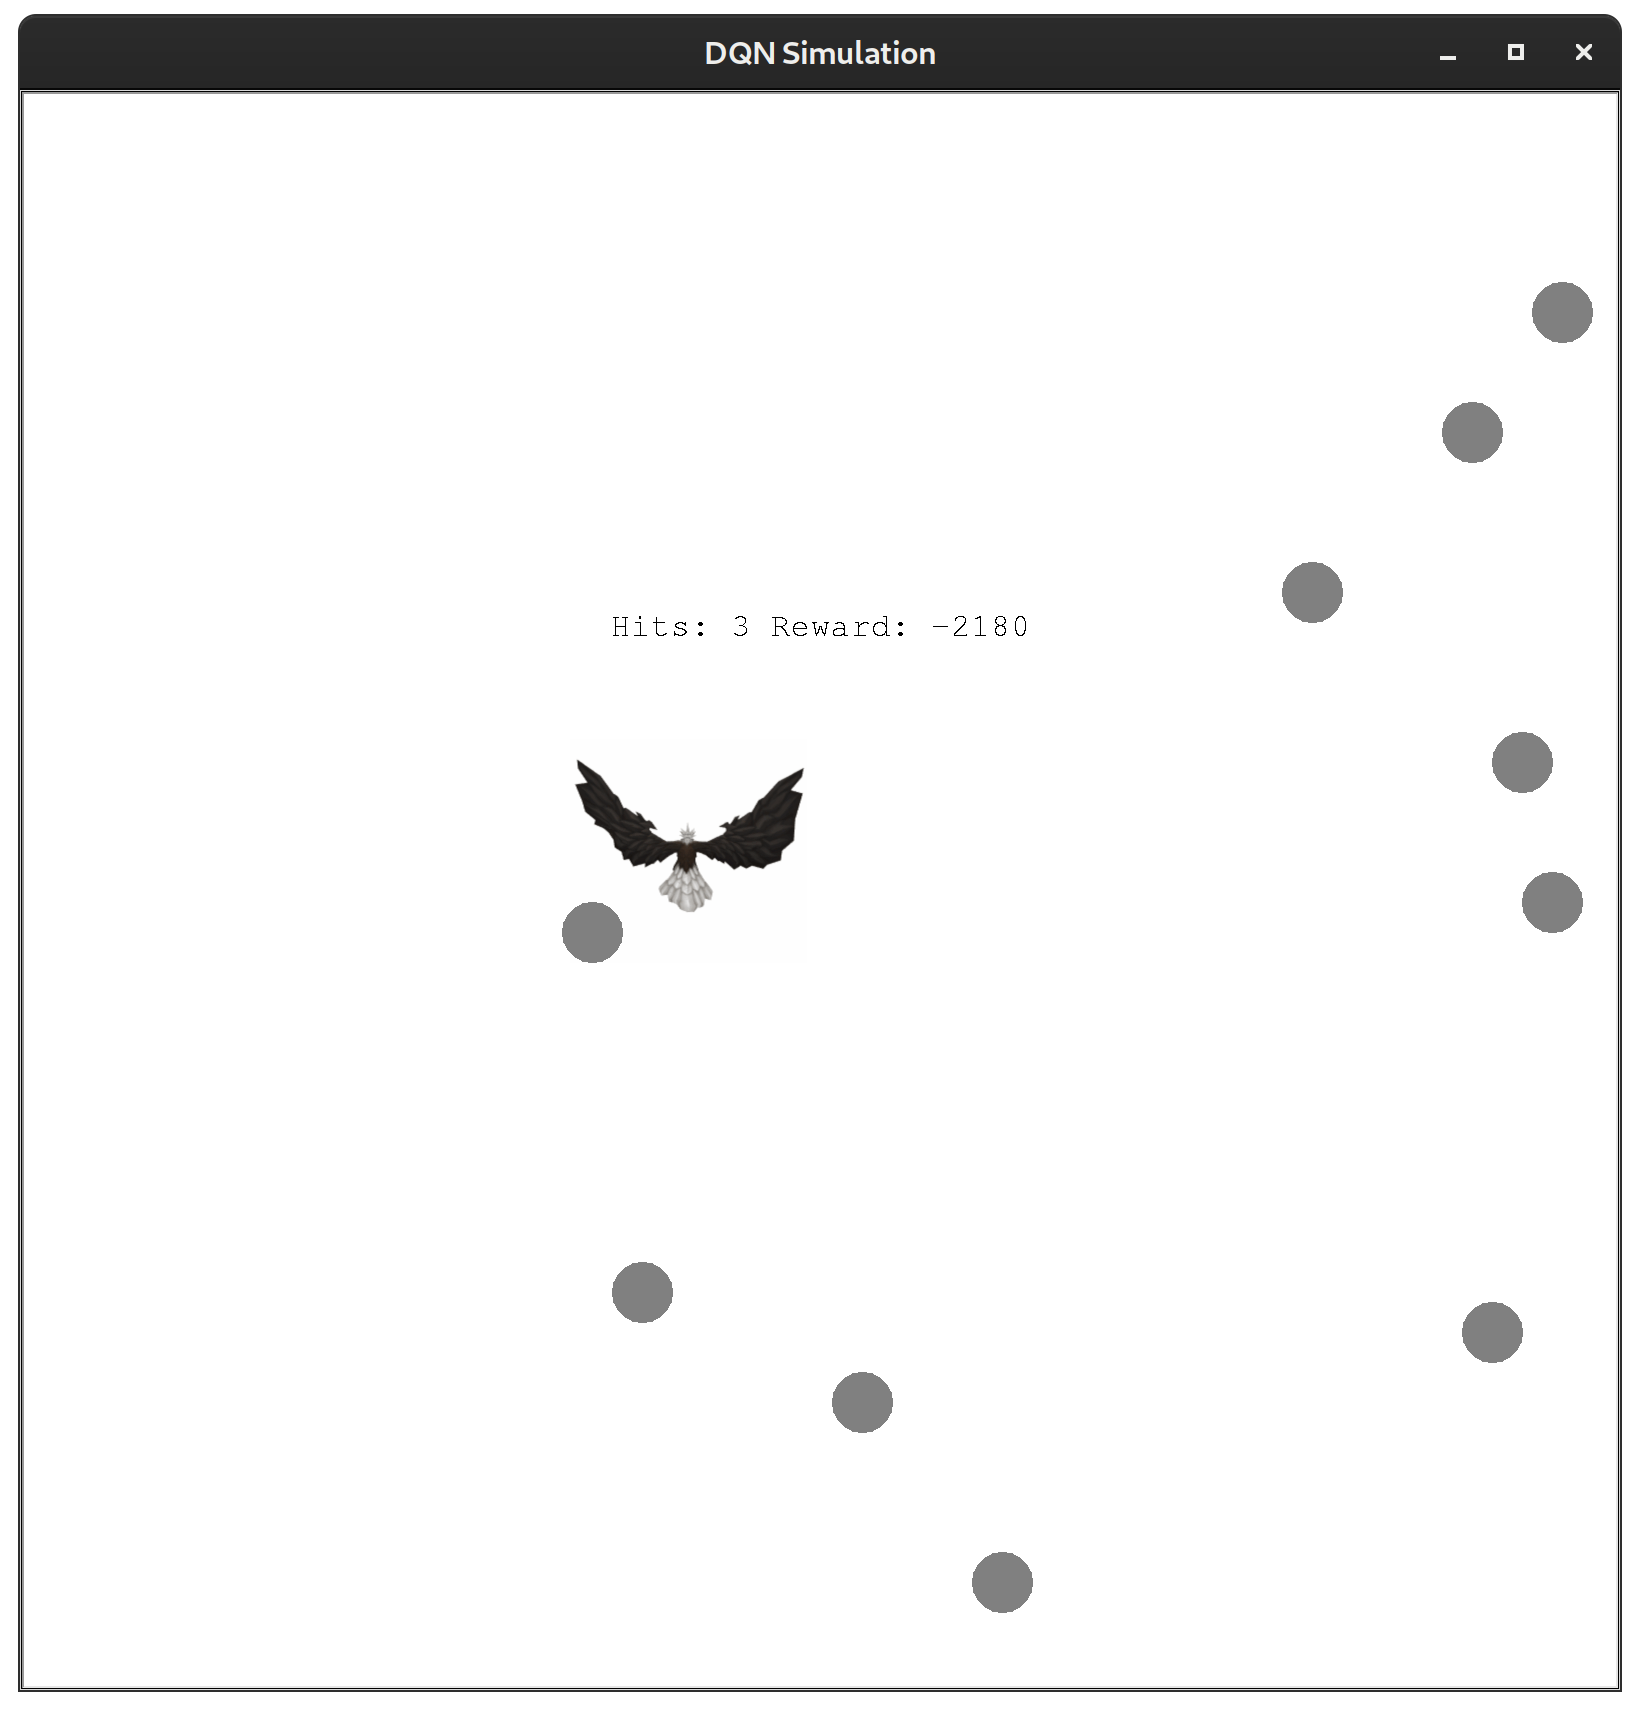
\includegraphics[scale=0.1]{figures/dqn_bird.png} 
  {\vskip 0cm Primer DQN okruženja za testiranje negativnih nagrada. Ptica je agent a sive tačke su nasumične prepreke koje treba izbeći. Implementacija sa Turtle Python modulom i Keras (Tensorflow) modelom.}
\end{figure}

\begin{figure}[!ht]
  \centering
  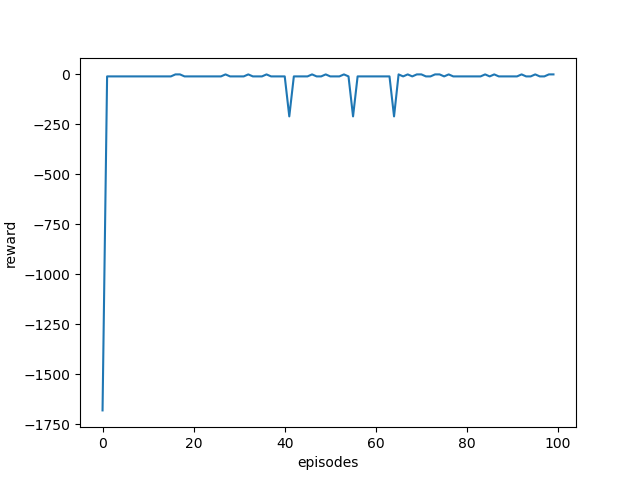
\includegraphics[scale=0.65]{figures/dqn_results.png} 
  {\vskip 0cm DQN nagrade za okruženje za izbegavanje prepreka. Model konvergira veoma brzo, nakon nekoliko epizoda dostiže nagradu $ 0 $. Iznenadni pad vrednosti nagrade predstavljaju nestavilnost modela zbog stohastičke prirode okruženja.}
\end{figure}

\subsection*{Zaključak}

Ova doktorska disertacija bavi se negativnim modelim negativnog učenja. Prikazani su i definisani novi i postojeći modeli uz dodatak modela koji kombiniju normalno i negativno učenje. Za CBOMF modele i modele sinergije pokazali smo da imaju veće performanse i robustnost u poređenju sa običnim modelima iste arhitekture.

U disertaciji su prikazani razni eksperimenti sa negacijom delova neuronskih mreža i kako se ove negacije mogu smisleno primeniti. Takođe su prikazane i razne modifikacije procesa treniranja neuronskih mreža koji nam omogućavaju da koristimo negativno učenje.

Za modele pravog negativnog učenja prikazane su dve implementacije: negativne sijamske neuronske mreže i negativni agenti pojačanog učenja gde smo prikazali da se i ovakvi modeli mogu produbiti i poboljšati negativnim učenjem.

Istraživanje predstavljeno u ovoj disertaciji predstavlja prve korake u novoj porodici dubokih neuronskih mreža za koje smo sigurni da će pronaći upotrebu u mnogim modernim sistemima.


